\chapter{Theoretical background}
\label{ch:introduction}

\section{The Standard Model}
\label{sec:standard_model}

The Standard Model (SM) is a theoretical framework in which 
the known elementary particles are expressed as excitations of relativistic
quantum fields\nomenclature{SM}{Standard Model}.
Particle interactions are determined by the Standard Model
Lagrangian, which is a function of these fields.
All of these fields are bosonic (having integer spin)
or fermionic (having half-integer spin), and the corresponding
particles are bosons and fermions.
This section briefly summarizes the Standard Model.  
A more detailed explanation may be found elsewhere \cite{griffiths,burgess,peskin}.

\subsection{Matter and forces}
\label{sec:forces}

\begin{table}
  \centering
  \renewcommand{\arraystretch}{1.5}
  \begin{tabular}{c|ccc|cc|c|c}
    \multirow{2}{*}{Fermion type} & \multicolumn{3}{c|}{Generation} & \multirow{2}{*}{$T$} & \multirow{2}{*}{$T_3$} & \multirow{2}{*}{$Y$} & \multirow{2}{*}{$Q$} \\
    & \nth{1} & \nth{2} & \nth{3} & & & & \\
    \hline \hline
    \multirow{2}{*}{Leptons} & $\doublet{\nu_e}{e}_{L}$ & $\doublet{\nu_\mu}{\mu}_{L}$ & $\doublet{\nu_\tau}{\tau}_{L}$  & $\frac{1}{2}$ & $\doublet{\frac{1}{2}}{-\frac{1}{2}}$ & $-1$ & $\doublet {0}{-1}$ \\
    & $e_{R}$ & $\mu_{R}$ & $\tau_{R}$ & $0$ & $0$ & $-2$ & $-1$  \\
    \hline
    \multirow{3}{*}{Quarks} & $\doublet{u}{d}_{L}$ & $\doublet{c}{s}_{L}$ & $\doublet{t}{b}_{L}$ & $\frac{1}{2}$ & $\doublet{\frac{1}{2}}{-\frac{1}{2}}$ & $\frac{1}{3}$ & $\doublet {\frac{2}{3}}{-\frac{1}{3}}$ \\
    & $u_{R}$ & $c_{R}$ & $t_{R}$ & $0$ & $0$ & $\frac{4}{3}$ & $\frac{2}{3}$  \\
    & $d_{R}$ & $s_{R}$ & $b_{R}$ & $0$ & $0$ & $-\frac{2}{3}$ & $-\frac{1}{3}$ \\
  \end{tabular}
  \caption{The three generations of fermions and their quantum numbers.  
    $T$ and $T_3$ represent total weak isospin and the third component 
    of weak isospin, respectively. $Y$ represents hypercharge.  $Q$ 
    represents electric charge.  
  }
  \label{tab:fermions}
  \renewcommand{\arraystretch}{1.0}
\end{table}

The Standard Model expresses particles of matter as spin-$1/2$ fermions
known as ``leptons'' and ``quarks.''  These particles and their properties
are listed in Table \ref{tab:fermions}.
Leptons include the massive and electrically charged electron ($e$), muon ($\mu$), and tau ($\tau$)
and their corresponding massless and electrically neutral neutrinos: $\nu_{e}$, $\nu_{\mu}$, and $\nu_{\tau}$.  
The extension of the Standard Model to include massive neutrinos
after the observation of neutrino flavor oscillations is discussed 
elsewhere \cite{standard-model-massive-neutrinos}.
Leptons are arranged into three ``generations.''  Each generation forms a 
doublet of left-handed states with non-zero weak isospin $\binom{\nu_\ell}{\ell}_{L}$ 
and a singlet of right-handed states $\ell_{R}$ with zero weak isospin.
In this context, right-handed fermions have parallel spin and momentum, while
left-handed fermions have anti-parallel spin and momentum.
Quarks include the up ($u$), down ($d$), charm ($c$), strange ($s$),
bottom ($b$), and top ($t$).  Like leptons, quarks
are arranged into three generations.  In the case of quarks, each generation
forms a doublet of left-handed states with non-zero weak isospin 
and two singlets of right-handed states with zero weak isospin.
Unlike leptons, quarks carry an additonal form of charge known as ``color'', which
has three values: red, green, and blue.

\begin{figure}[htbc]
  \begin{center}
    %
% Sketch of the SM particles and interactions
%
\begin{tikzpicture}
  [x=16cm,y=8cm,node distance=2cm,auto,
    every loop/.style={},
    % particle/.style={circle,draw=blue!50,fill=blue!20,thick}]
    particle/.style={circle,draw=black!50,fill=white!20,thick}]
  % Particles
  \node[particle] at (4cm,7cm) (L) {$\Plepton^{\pm}$};
  \node at (3cm,9cm) (leptons) {  % table with leptons
    \begin{tabular}{ccc}
      \multicolumn{3}{c}{Leptons (\Pneutrino, $\Plepton^{\pm}$)} \\
      \hline 
      \Pnue & \Pnum & \Pnut \\
      \Pe & \Pmu & \Ptau \\
    \end{tabular}
  };
  \node[right of=L] (dummyRL) {};
  \node[right of=dummyRL] (dummyRRL) {};
  \node[below left of=L] (dummyBL) {};
  \node[particle] (Q) [right of=dummyRRL]{\Pquark};
  \node at (10cm,9cm) (quarks) {  % table with quarks
    \begin{tabular}{ccc}
      \multicolumn{3}{c}{Quarks (\Pquark)} \\
      \hline
      \Pup & \Pcharm & \Ptop \\
      \Pdown & \Pstrange & \Pbottom \\
    \end{tabular}
  };
  \node[particle] (L2) [above left of=dummyBL]{\Pneutrino};
  \node[particle] (P) [below left of=dummyBL]{\Pphoton};
  \node[particle] (W) [below right of=dummyBL]{\PW};
  \node[particle] (Z) [right of=W]{\PZ};
  \node[right of=Z] (dummyRZ) {};
  \node[particle] (G) [right of=dummyRZ]{\Pgluon};
  \node[below of=P] (dummyBP) {};
  \node[particle] (H) [below right of=dummyBP]{\PH};

  % Interactions
  \path
  (L)  edge [bend right] (P)
  (L)  edge [bend right] (H)
  (L)  edge [bend left] (W)
  (L)  edge [bend left] (Z)
  (L2)  edge [bend left] (H)
  (L2)  edge [bend left] (W)
  (L2)  edge [bend left] (Z)
  % (L2)  edge [bend left] (L)
  (Q) edge [bend right=20] (P)
  (Q) edge [bend right=20] (W)
  (Q) edge [bend right=20] (Z)
  (Q) edge [bend left=20] (G)
  (Q) edge [bend left=20] (H)
  (P) edge [bend right] (W)
  (W) edge [loop above] (W)
  (W) edge [bend right] (Z)
  (W) edge [bend left] (H)
  (Z) edge [bend left=20] (H)
  (H) edge [loop below] (H)
  (G) edge [loop below] (G);

  % Draw curly braces using path decoration
  \draw [gray,decorate,decoration={brace,amplitude=5pt}]
  (-0.25cm,6.25cm) -- (-0.25cm,7.75cm)
  node [black,midway,below=0pt,xshift=-2pt,rotate=-90] {Spin 1/2};
  \draw [gray,decorate,decoration={brace,amplitude=5pt}]
  (-0.25cm,3.25cm) -- (-0.25cm,4.75cm)
  node [black,midway,below=0pt,xshift=-2pt,rotate=-90] {Spin 1};
  \draw [gray,decorate,decoration={brace,amplitude=5pt}]
  (-0.25cm,0.00cm) -- (-0.25cm,1.5cm)
  node [black,midway,below=0pt,xshift=-2pt,rotate=-90] {Spin 0};
  % Draw mass scales
  \draw (5.40cm,-0.30cm) rectangle (13.10cm,1.5cm); % draw the box
  \draw[->,xshift=5.5cm] (0cm,0.5cm) -- coordinate (x axis mid) (7.5cm,0.5cm);
  \node[below=0.10cm, xshift=3.25cm] at (x axis mid) {mass};
  \foreach \x/\text in {1/meV, 2/eV,3/keV,4/MeV,5/GeV,6/TeV }
      \draw [xshift=5.0cm,yshift=0.5cm](\x cm,1pt) -- (\x cm,-3pt)
      node[anchor=north] {\text};
  % \node[draw=blue,inner sep=0pt,thick,circle,fit=(x axis mid)] {}; % test fit feature box
  % should enter the mass values and actually compute the log to get x...
  \node [text height=10pt] at (5.0cm+1.5cm,0.7cm +2pt) (mnu) {\Pnue,\Pnum,\Pnut};
  \node [text height=10pt] at (5.0cm+3.5cm,0.7cm +2pt) (mel) {\Pe};
  \node [text height=10pt] at (5.0cm+4.5cm,0.7cm +2pt) (mmu) {\Pmu};
  \node [text height=10pt] at (5.0cm+5.05cm,0.7cm+2pt) (mtau) {\Ptau};
  \node [text height=10pt] at (5.0cm+3.8cm,0.7cm+12pt) (mud) {$\Pup\Pdown$};
  \node [text height=10pt] at (5.0cm+4.5cm,0.7cm+12pt) (ms) {\Pstrange};
  \node [text height=10pt] at (5.0cm+5.05cm,0.7cm+12pt) (mcb) {$\Pcharm\Pbottom$};
  \node [text height=10pt] at (5.0cm+5.75cm,0.7cm+12pt) (mt) {\Ptop};

\end{tikzpicture}


  \end{center}
  \caption{\label{fig:smParticles} 
    Schematic view of the Standard Model particles and of their interactions. 
    Connecting lines represent interactions between particles.  
    The masses of the fundamental constituents are indicated in the bottom-right inset.}
\end{figure}

Leptons and quarks interact with each other via the exchange of spin-$1$ bosons.
These bosons include the gluon ($g$), the $W$ and $Z$ bosons, and the photon ($\gamma$).
They are responsible for the three forces described by the Standard Model:
the strong force, the weak force, and electromagnetism, respectively.  
A fourth force, gravity, is not described by the Standard Model, but its effects
are negligable when compared to the effects of the other three forces 
on the sub-atomic particle mass scale.
The interactions between these spin-$1$ bosons and the spin-$1/2$ fermions 
(along with boson-boson interactions) are shown 
in the schematic in Figure \ref{fig:smParticles}.  The three forces described by 
the Standard Model are discussed in greater detail below.

Electromagnetism influences particles that carry electric charge.  This influence
is manifested via the exchange of a photon, and the theory describing it
is known as Quantum Electrodynamics (QED)\nomenclature{QED}{Quantum electrodynamics}.
Electromagnetism was the first of the forces in the Standard Model to be discovered,
and the strong and weak forces are named for their coupling strengths relative to 
electromagnetism.  Because the photon is massless, the range of electromagnetism 
is infinite.

The weak force influences all fermions via the exchange of $W$ and $Z$ bosons.
The strength of the weak force is roughly $10^{-5}$ that of electromagnetism,
and it has several distinctive properties.  First, the weak force behaves differently
for fermions with different chiralities.  Namely, the charged $W$ boson only interacts 
with fermions that have left-handed chirality (i.e. leptons and quarks having 
non-zero weak isospin) and their right-handed anti-particles. The neutral $Z$ boson interacts 
with fermions and anti-fermions of both right and left-handed chiralities.  Second, because 
the $W$ and $Z$ bosons are massive ($M \sim 100$~\GeV), the weak force has a short 
range ($R \sim 10^{-18}$~m).  The mass associated with these bosons is explained by the Higgs mechanism.
Finally, the weak force is the only force with the ability to change the flavor of quarks.

The strong force influences particles that carry a color charge.  This influence is
manifested via the exchange of gluons: electrically neutral and massless spin-$1$ bosons that carry 
a color charge themselves.
Only quarks and gluons themselves are known 
to carry color charge, so the strong force influences only these particles.  
The theory describing the interaction between quarks and gluons is  known as Quantum Chromodynamics (QCD).
\nomenclature{QCD}{Quantum chromodynamics} 
The strength 
of the strong force is roughly 100 times that of electromagnetism, and it is the only force 
that does not decrease in strength as the distance between the two interacting particles increases.  
As a result, it is energetically favorable for a quark-antiquark pair to be created from the 
vacuum rather than for isolated quarks to interact over long distances.  This means that 
isolated quarks are rarely observed.  Instead, quarks are nearly always observed as a 
constituent of other non-fundamental, color charge-neutral particles called ``hadrons.''
\footnote{The exception is the top quark, which has a mean lifetime 20 times shorter 
than the timescale for strong force interactions and does not hadronize.}  
A similar effect is observed in the case of gluons, which also hadronize and are never observed in isolation.
This property is called ``confinement.''  
It should be noted that the residual strong force interaction
between color charge-neutral hadrons is not zero, and it has a short range 
($R \sim 10^{-15}$~m).

In the context of collider physics, hadronizing quarks and gluons produced 
in particle collisions result in a collimated spray of hadrons, which are called ``jets''.
The reconstruction of the original quark and gluon energy and momentum from jets is a critical
challenge of collider physics, and it is discussed in further detail in Section \ref{sec:jetmet}.

\subsection{Gauge invariance and the Higgs mechanism}

In general, a Lagrangian is said to be gauge invariant (or to have a gauge symmetry)
if it remains invariant under a continuous gauge transformation.  
A central postulate of the Standard Model Lagrangian in particular is that the
dynamics of all particles are determined by specifying underlying local gauge symmetries.
This implies that the forces described in the Standard Model are associated with symmetry groups.
The strong force is associated with the $\text{SU}(3)_{C}$ symmetry group, where
$C$ corresponds to color.
Gauge symmetries allow for the electromagnetic and weak forces to be unified into a single ``electroweak'' interaction
associated with the direct product of the $\text{SU}(2)_{L}$ and $\text{U}(1)_{Y}$ symmetry 
groups \cite{glashow,weinberg,salam:1968}, where 
$L$ corresponds to left-handed chirality and $Y$ corresponds to weak hypercharge.
The combined symmmetry group of the Standard Model Lagrangian is therefore 
$\text{SU}(3)_{C} \times \text{SU}(2)_{L} \times \text{U}(1)_{Y}$.

The concept of local gauge invariance allows
for the unification of the electromagnetic and weak forces 
and predicts the existence of the $W$ and $Z$ bosons,
which had not been observed when the theory was originally described.
However, local gauge invariance also requires all 
fermions and gauge bosons to be massless, which is clearly
at odds with various experimental results.  This shortcoming was 
addressed independently by multiple groups in 1964 via what is now 
called the ``Higgs mechanism'' \cite{higgs,englert,guralnik}.
The Higgs mechanism introduces a fundamental, self-interacting,
spin-$0$ field that permeates all of space.
This field, the Higgs field, interacts with the $W$ and $Z$ bosons
associated with the $\text{SU}(2)_{L} \times \text{U}(1)_{Y}$ 
symmetry group and all fermions.  
The quantum of the Higgs field is the Higgs boson, $H$.
The Higgs field is given a non-zero vacuum expectation value, $v$, the value of which
is determined from experiment. 
The non-zero vacuum expectation value results in a spontaneous breaking of the 
$\text{SU}(2)_{L} \times \text{U}(1)_{Y}$ symmetry and imparts mass
to the $W$ and $Z$ bosons and the charged fermions (neutrinos, the photon, and the gluon
remain massless).  The Higgs field, the Higgs boson, and the Higgs
mechanism are therefore all essential components of the Standard Model.

\subsection{Limitations of the Standard Model}

The success of the Standard Model has been remarkable.
All of the particles described in the previous sections have been 
observed.  Their properties and interactions behave in accordance 
with Standard Model predictions down to a length scale of 
approximately $10^{-18}$~m.  In spite of this success, however, the 
Standard Model is incomplete.  

The Standard Model's failure to address gravity as a fundamental
force means that it is unable to describe interactions at the Planck 
scale ($M_{\text{Planck}} \approx 1.22 \times 10^{19}$), at which
point the quantum effects of gravity become too large to ignore.
The Standard Model also fails to explain why the gap between the Planck
scale and the electroweak scale is so large: the weak force is roughly 
$10^{32}$ times stronger than gravity
(an issue known as the ``hierarchy problem'').
Other unanswered questions trouble the Standard Model at lower energy
scales than the Planck scale.  Experimental results from
astrophysics suggest that roughly one quarter of the energy density of the
universe is composed of ``dark matter'' while nearly three quarters 
is composed of ``dark energy''.  However, the Standard Model makes no predictions
as to the composition of dark matter, nor does it contain any dark
matter particle candidates (i.e. massive, neutral, stable, fundamental particles).
In addition, the precise nature of neutrino oscillation and neutrino masses
is unknown.  Most importantly for this thesis, the Standard Model does not 
explain the presence of three generations of fermions (see Table \ref{tab:fermions}), nor
does it explain the similarity of the arrangements of quarks and leptons under the electroweak interaction.

The presence of these unanswered questions in spite of undeniable 
experimental success leads many to suspect that the Standard Model
is a low energy remnant of a larger theory.  The nature of this larger
theory and various ``extensions'' to the Standard Model are the subject
of intense speculation in the particle physics community.
Leptoquarks, the subject of this thesis, form the basis of 
one such extension of the Standard Model.  They are discussed in the following 
section.

\section{Leptoquarks}

In the Standard Model, leptons and quarks are formally independent 
from each other.  However, both leptons and quarks come in three generations, 
and they are similarly arranged in multiplets under the electroweak interaction
(see Table \ref{tab:fermions}).  This arrangement is necessary for the
cancellation of triangle anomalies, which in turn is necessary for the 
Standard Model to be a consistent quantum field theory \cite{lq-classification}.

A possible motivation for this similarity comes from considering a hypothetical
interaction between leptons and quarks.  This interaction would include one or more 
bosonic fields interacting between leptons and quarks.  Such fields, known as leptoquarks 
(LQ)\nomenclature{LQ}{Leptoquarks},
would form as color triplets under $\text{SU}(3)_{C}$,
carry both lepton number ($L$) and baryon number ($B$),
and carry fractional charge ($Q$).  Other properties, including 
spin, weak isospin, specific electric charge, and fermion number 
($F = 3B+L$) are model-dependent.

Leptoquarks are motivated by many theories beyond the Standard Model.
Some examples include 
Grand Unified Theories (GUTs)\nomenclature{GUT}{Grand unified theory} based
on gauge groups including 
Pati-Salam SU(4) color symmetry \cite{pati-salam-su4-1,pati-salam-su4-2},
SU(5)  \cite{su5-1,su5-2},
SO(10) \cite{su10-1,su10-2},
and SU(15) \cite{su15-1,su15-2}.
Other examples include superstring-inspired $\text{E}_6$ models \cite{superstring_e6},
extended technicolor models \cite{technicolor1,technicolor2,technicolor3},
composite models \cite{composite-1,composite-2},
horizontal symmetry theories \cite{horizontal},
strongly coupled weak-interaction models \cite{strongweak},
and R-parity violating supersymmetric models \cite{rpv1,rpv2,rpv3}.

In practice, searches for leptoquarks at colliders are performed
using general effective models which avoid these inconsistencies between various models.
The most popular of these effective models is the 
Buchm{\"u}ller-R{\"u}ckl-Wyler effective leptoquark model, which is described
in the following section.

\subsection{Buchm{\"u}ller-R{\"u}ckl-Wyler effective leptoquark model}
\label{sec:brw-model}

The general effective model used in this thesis was proposed in 1987 by
Buchm{\"u}ller, R{\"u}ckl, and Wyler \cite{mBRW1} (BRW model)\nomenclature{BRW}{Buchm{\"u}ller, R{\"u}ckl, Wyler model of leptoquarks}.
The four underlying assumptions of the BRW model are:
{\bf 1)} leptoquarks have renormalizable interactions (their couplings to Standard Model lepton-quark pairs are dimensionless),
{\bf 2)} leptoquark interactions are invariant under the Standard Model gauge groups: $\text{SU}(3)_{C} \times \text{SU}(2)_{L} \times \text{U}(1)_{Y}$,
{\bf 3)} leptoquarks couple {\it only} to Standard Model fermions and gauge bosons, and 
{\bf 4)} leptoquarks conserve lepton number ($L$) and baryon number ($B$) separately in order to protect against rapid proton decay.  

Under these four initial assumptions underlying the BRW model, leptoquarks are permitted
to decay to any combination of leptons and quarks.  This can lead to
tree-level flavor-changing neutral current (FCNC)\nomenclature{FCNC}{Flavor-changing neutral current} 
decays.  An example of such a tree-level FCNC decay is shown in Figure 
\ref{fig:feynman_LO_FD_FCNC_LQ}.  To protect against these decays, 
the BRW model may be augmented with the additional requirement {\bf 5)} that leptoquarks
may only couple to fermions of a single generation\footnote{While the requirement that 
leptoquarks only couple to a single fermion generation is traditional, requiring 
that leptoquarks do not couple to more than one generation of leptons and more
than one generation of quarks is enough to protect against tree-level 
FCNC decays like the one shown in Figure \ref{fig:feynman_LO_FD_FCNC_LQ}.
For example, a leptoquark could be allowed to couple to first generation
leptons and third generation quarks.}.
This thesis is focused on first generation leptoquarks (leptoquarks coupling to electrons,
electron neutrinos, up quarks, and down quarks) specifically.
\begin{figure}
  \centering
  \begin{subfigure}[b]{0.30\textwidth}
    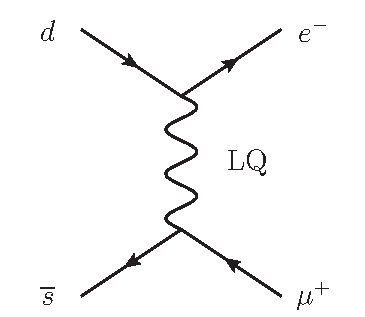
\includegraphics[width=\textwidth]{tex/theory/fig/kaon_lq1}
    \caption{}
    \label{fig:feynman_LO_FD_FCNC_LQ_a}
  \end{subfigure}
  \begin{subfigure}[b]{0.30\textwidth}
    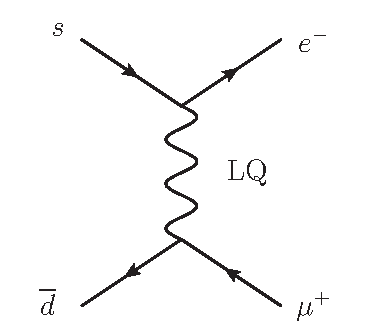
\includegraphics[width=\textwidth]{tex/theory/fig/kaon_lq2}
    \caption{}
    \label{fig:feynman_LO_FD_FCNC_LQ_b}
  \end{subfigure}
  \caption{
    Examples of a tree-level FCNC and lepton flavor violating 
    decay $K^{0}_{L}(d\overline{s}+s\overline{d}) \rightarrow e^{-}\mu^{+}$, mediated
    by a vector leptoquark.
    This decay mode is permitted by some leptoquark models \cite{pati-salam-su4-1,pati-salam-su4-2}
    but forbidden by the Standard Model.
  }
  \label{fig:feynman_LO_FD_FCNC_LQ}
\end{figure}
Other low energy constraints, such as chirally suppressed meson decays
(for example, $\pi \rightarrow e\nu$ as shown in Figure \ref{fig:feynman_LO_FD_pion})
make it necessary to introduce a requirement {\bf 6)} that leptoquarks have
purely chiral couplings.
The addition of requirements {\bf 5} and {\bf 6} to the BRW model results in the 
minimal Buchm{\"u}ller-R{\"u}ckl-Wyler effective model 
(mBRW)\nomenclature{mBRW}{minimal Buchm{\"u}ller-R{\"u}ckl-Wyler model of leptoquarks}.

\begin{figure}
  \centering
  \begin{subfigure}[b]{0.45\textwidth}
    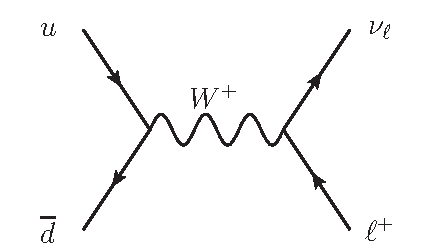
\includegraphics[width=\textwidth]{tex/theory/fig/pion_w}
    \caption{}
    \label{fig:feynman_LO_FD_pion_w}
  \end{subfigure}
  \begin{subfigure}[b]{0.30\textwidth}
    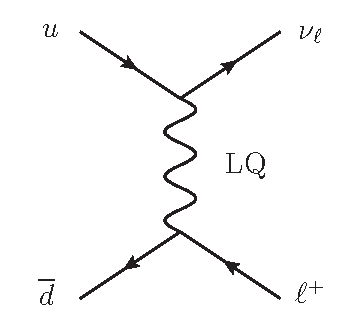
\includegraphics[width=\textwidth]{tex/theory/fig/pion_lq}
    \caption{}
    \label{fig:feynman_LO_FD_pion_LQ}
  \end{subfigure}
  \caption{
    Example of a pion decay, $\pi^{+} \rightarrow \ell^{+}\nu$, mediated
    by a Standard Model $W^{+}$ boson (a) and a vector leptoquark (b) \cite{pati-salam-su4-1,pati-salam-su4-2}. 
    The decay $\pi^{+} \rightarrow e^{+}\nu$ is chirally suppressed by the Standard Model but
    not by some leptoquark models.
  }
  \label{fig:feynman_LO_FD_pion}
\end{figure}

These requirements lead to seven scalar and seven vector leptoquarks.
These leptoquarks may be classified by fermionic number, $F = 3B + L$, such that $|F| = 0$ or 2.
The interactions between mBRW leptoquarks and Standard Model fermions 
are described by the following Lagrangian:
\begin{equation}
  \mathcal{L} = \mathcal{L}_{|F|=2} + \mathcal{L}_{F=0} \\
  \label{eqn:brw-lagrangian-simple}
\end{equation}
\noindent The terms $\mathcal{L}_{|F|=2}$ and $\mathcal{L}_{F=0}$ given in 
Equation \ref{eqn:brw-lagrangian-simple} may be defined as follows:
\begin{equation}
  \begin{aligned}
    \mathcal{L}_{|F|=2} 
    &= ( g_{1L} \overline{q}_{L}^{c} i \tau_2 \ell_{L} + g_{1R}\overline{u}_{R}^{c} e_{R}) S_{0} \\
    &+ ( \tilde{g}_{1R} \overline{d}^{c}_{R} e_{R} ) \tilde{S}_{0} \\
    &+ ( g_{3L} \overline{q}_{L}^{c} i \tau_2 \vec{\tau} \ell_{L} ) \vec{S}_{1} \\
    &+ ( g_{2L} \overline{d}_{R}^{c} \gamma ^{\mu} \ell_{L} + g_{2R} \overline{q}_{L}^{c} \gamma^{\mu} e_{R} ) V_{\frac{1}{2}\mu} \\
    &+ ( \tilde{g}_{2L} \overline{u}_{R}^{c} \gamma^{\mu} \ell_{L})\tilde{V}_{\frac{1}{2}\mu} \\ 
    &+ \text{h.c.} \\
  \end{aligned}
  \label{eqn:brw-lagrangian-f2}
\end{equation}
\begin{equation}
  \begin{aligned}
    \mathcal{L}_{F=0} 
    &= (h_{2L} \overline{u}_{R} \ell_{L} + h_{2R} \overline{q}_{L} i \tau_{2} e_{R}) S_{\frac{1}{2}} \\
    &+ (\tilde{h}_{2L} \overline{d}_{R} \ell_{L}) \tilde{S}_{\frac{1}{2}} \\
    &+ (h_{1L} \overline{q}_{L} \gamma^{\mu} \ell_{L} + h_{1R} \overline{d}_{R} \gamma^{\mu} e_{R}) V_{0\mu} \\
    &+ (\tilde{h}_{1R} \overline{u}_{R} \gamma^{\mu} e_{R}) \tilde{V}_{0\mu} \\
    &+ (h_{3L} \overline{q}_{L} \vec{\tau}\gamma^{\mu}\ell_{L} ) V_{1\mu} \\ 
    &+ \text{h.c.}
  \end{aligned}
  \label{eqn:brw-lagrangian-f0}
\end{equation}
Equations \ref{eqn:brw-lagrangian-f2} and \ref{eqn:brw-lagrangian-f0} are given in the {\it Aachen} notation 
\cite{mBRW-aachen}. Scalar leptoquarks are denoted with an $S$ and vector leptoquarks with a $V$.  
The subscripts on $S$ and $V$ denote 
the $\text{SU}(2)_{L}$ isospin (0, 1/2, 1).
The $\sim$ symbol over ${\tilde S}$ and ${\tilde V}$ is purely a label for distinguishing 
between two distinct leptoquarks with identical spin and weak isospin but different hypercharge
(for example $S_0$ and ${\tilde S}_{0}$).
$q_{L}$ and $\ell_{L}$ represent the $SU(2)_{L}$ left-handed doublets for quarks and leptons.
$e_{R}$, $u_{R}$, and $d_{R}$ represent the right-handed lepton, up-type quark, and down-type quark singlets, respectively.
$\tau_{i}$ represent the Pauli matrices. $\gamma^\mu$ represent the Dirac matrices.  
$g$, $h$, ${\tilde g}$, and ${\tilde h}$ are coupling constants: the subscripts denote 
the dimension of the $\text{SU}(2)_{L}$ representation (1, 2, 3) of the coupled leptoquark and
the chirality of the coupled lepton ($L$, $R$).  It is traditional to write these 
couplings as $\lambda_{R} = g_{R},h_{R}$ and $\lambda_{L} = g_{L},h_{L}$.
The $\psi^{c}$ operators are the charge conjugate of the fermion fields, such that $\psi^{c} \equiv C \overline{\psi}^{T}$.
For simplicity, color, weak isospin, and generation (flavor) indices are omitted.\footnote{
In the notation used by the original BRW paper \cite{mBRW1}, leptoquarks with different 
fermionic number or spin are given distinct symbols ($R$, $S$, $U$, $V$).  The subscript of those symbols corresponds
to the dimension of the leptoquark's $\text{SU}(2)_{L}$ representation (1, 2, 3).
In the {\it Aachen} notation \cite{mBRW-aachen}, leptoquarks with different spin are given 
distinct symbols ($S$, $V$).  The subscript of those symbols corresponds to the leptoquark's 
$\text{SU}(2)_{L}$ isospin ($0$, $1/2$, $1$).
The two notations have the following correspondence:
$S_{0}\leftrightarrow S_{1}^{\text{BRW}}$;
${\tilde S}_{0}\leftrightarrow {\tilde S_{1}}^{\text{BRW}}$;
$S_{1/2}\leftrightarrow R_{2}^{\text{BRW}}$;
${\tilde S}_{1/2}\leftrightarrow {\tilde R}_{2}^{\text{BRW}}$;
$S_{1}\leftrightarrow S_{3}^{\text{BRW}}$;
$V_{0}\leftrightarrow U_{1}^{\text{BRW}}$;
${\tilde V}_{0}\leftrightarrow {\tilde U}_{1}^{\text{BRW}}$;
$V_{1/2}\leftrightarrow V_{2}^{\text{BRW}}$;
${\tilde V}_{1/2}\leftrightarrow {\tilde V}_{2}^{\text{BRW}}$;
$V_{1}\leftrightarrow U_{3}^{\text{BRW}}$.}

Some of the properties of the leptoquarks given by this Lagrangian
are listed in Table \ref{tab:lq-classification},
including the leptoquarks' total weak isospin, third component 
of weak isospin, hypercharge, electric charge, fermionic number, coupling constants,
and decay modes.
The leptoquark symbols ($S$ and $V$) in Table \ref{tab:lq-classification} have
an additional subscript beyond those used in the Lagrangian.  
This subscript corresponds to the chirality ($L$, $R$)
of the lepton to which the leptoquark is coupled.
For most experimental searches (including this one), mass degeneracy is assumed within each
isospin family.  The theoretical motivation behind this assumption is that one
would expect all leptoquarks within a given $SU(2)_{L}$ representation to be degenerate,
ignoring loop corrections.  For simplicity, therefore, each leptoquark symbol corresponds
to a single isospin family, including all of the electric charge possibilities within that family.
For example, the symbol $V_{1,L}$ corresponds to any of the three vector leptoquarks that 
have total weak isospin $T = 1$, couple to a left handed lepton,
 and have electric charge $Q = -5/3$, $-2/3$, or $1/3$.  By construction, the decay branching
ratios $\beta = \text{BR}(\text{LQ}\rightarrow\ell^{\pm} q)$ of each of these leptoquarks into a final state
containing a charged lepton and a quark are fixed to 0, $1/2$, or 1 \cite{mBRW2}.

\begin{table}
  \centering
  \renewcommand{\arraystretch}{1.5}
  \begin{tabular}{cc|cc|c|c|c|ccc|c}
    LQ & squark & $T$ &  $T_{3}$ & $Y$ & $Q$     & $F$ & $\lambda_{L} (lq)$ & $\lambda_{R} (lq)$& $\lambda_{L} (\nu q)$  & Decay mode \\
    \hline\hline    
    $S_{0,L}$ & ${\bar{\tilde d}}_{R}$  & $0$ & $0$     & $2/3$ & $1/3$  & $-2$ & $g_{1L}$ & 0 & $-g_{1L}$ & $e_{L}^{+}\overline{u}_{L}$, $\overline{\nu}_{L}\overline{d}_{L}$ \\
    \hline
    $S_{0,R}$ & - & $0$ & $0$     & $2/3$ & $1/3$  & $-2$ & 0 & $g_{1R}$ & 0 & $e_{R}^{+}\overline{u}_{R}$                \\
    \hline
    $\tilde{S}_{0,R}$ & - & $0$ & $0$ & $8/3$ & $4/3$ & $-2$ & 0 & ${\tilde g}_{1R}$ & 0 & $e_{R}^{+}\overline{d}_{R}$           \\
    \hline
    \multirow{2}{*}{$S_{\frac{1}{2},L}$} & - & \multirow{2}{*}{$1/2$} 
    & $1/2$ & \multirow{2}{*}{$7/3$} & $5/3$ & \multirow{2}{*}{0} & $h_{2L}$ &0 & 0 & $e_{L}^{+} u_{L}$     \\
    & - & & $-1/2$  & & $2/3$ & & 0  & 0 & $h_{2L}$ & $\overline{\nu}_{L}u_{L}$   \\
    \hline
    \multirow{2}{*}{$S_{\frac{1}{2},R}$} & - & \multirow{2}{*}{$1/2$}
    & $1/2$ & \multirow{2}{*}{$7/3$} & $5/3$ & \multirow{2}{*}{$0$} & 0 & $h_{2R}$ & 0 & $e_{R}^{+}u_{R}$     \\
    & - & & $-1/2$  & & $2/3$ & & 0 & $-h_{2R}$ & 0 & $e_{R}^{+}d_{R}$     \\
    \hline
    \multirow{2}{*}{$\tilde{S}_{\frac{1}{2},L}$} & ${\tilde u}_{L}$ & \multirow{2}{*}{$1/2$} 
    & $1/2$ & \multirow{2}{*}{$1/3$} & $2/3$ & \multirow{2}{*}{$0$} & ${\tilde h}_{2L}$ & 0 & 0 & $e_{L}^{+}d_{L}$     \\
    & ${\tilde d}_{L}$ & & $-1/2$  & & $-1/3$ & &0 & 0 &${\tilde h}_{2L}$ & $\overline{\nu}_{L}d_{L}$   \\
    \hline
    \multirow{3}{*}{$S_{1,L}$} & - & \multirow{3}{*}{1}
    & $1$   & \multirow{3}{*}{$2/3$} & $4/3$ & \multirow{3}{*}{$-2$} &$-\sqrt{2}g_{3L}$ &0 &0 & $e_{L}^{+}\overline{d}_{L}$  \\
    & - & & $0$    & & $1/3$ &  & $-g_{3L}$ & 0 & $-g_{3L}$ & $e_{L}^{+}\overline{u}_{L}$, $\overline{\nu}_{L}\overline{d}_{L}$ \\
    & - & & $-1$    & & $-2/3$  &  & 0 & 0 & $\sqrt{2}g_{3L}$ & $\overline{\nu}_{L}\overline{u}_{L}$              \\
    \hline\hline    
    $V_{0,L}$  & - & $0$ & $0$  & $4/3$ & $2/3$ & $0$ & $h_{1L}$ &0  & $h_{1L}$ &  $e_{L}^{+}d_{R}$, $\overline{\nu}_{L}u_{L}$ \\
    \hline
    $V_{0,R}$  & -  & $0$ & $0$  & $4/3$ & $2/3$ & $0$ & 0 & $h_{1R}$ & 0 & $e_{R}^{+}d_{L}$ \\
    \hline
    $\tilde{V}_{0,R}$  & -  & $0$ & $0$  & $10/3$ & $5/3$ & $0$ & 0 & ${\tilde h}_{1R}$ & 0 & $e_{R}^{+}u_{L}$ \\
    \hline
    \multirow{2}{*}{$V_{\frac{1}{2},L}$} & - & \multirow{2}{*}{$1/2$}
    &   $1/2$ & \multirow{2}{*}{$5/3$} & $4/3$ & \multirow{2}{*}{$-2$} & $g_{2L} $ & 0 & 0 & $e_{L}^{+}\overline{d}_{R}$ \\
    & - & & $-1/2$  & & $1/3$ & & 0 & 0 & $g_{2L}$ & $\overline{\nu}_{L}\overline{d}_{R}$ \\
    \hline
    \multirow{2}{*}{$V_{\frac{1}{2},R}$} & - & \multirow{2}{*}{$1/2$} 
    &  $1/2$ &\multirow{2}{*}{$5/3$} & $4/3$ & \multirow{2}{*}{$-2$} & 0 & $g_{2R}$ & 0 & $e_{R}^{+}\overline{d}_{L}$ \\
    & - & & $-1/2$ & & $1/3$ & &0  & $g_{2R}$& 0 &  $e_{R}^{+}\overline{u}_{L}$ \\
    \hline
    \multirow{2}{*}{$\tilde{V}_{\frac{1}{2},L}$} & - & \multirow{2}{*}{$1/2$}
    & $1/2$ & \multirow{2}{*}{$-1/3$} & $1/3$ & \multirow{2}{*}{$-2$} & ${\tilde g}_{2L}$  & 0 & 0 & $e_{L}^{+}\overline{u}_{R}$ \\
    & - & & $-1/2$ & & $-2/3$ & & 0 & 0 & ${\tilde g}_{2L}$ &  $\overline{\nu}_{L}\overline{u}_{R}$ \\
    \hline
    \multirow{3}{*}{$V_{1,L}$} & - & \multirow{3}{*}{$1$} 
    &  $1$   & \multirow{3}{*}{$4/3$} & $5/3$ & \multirow{3}{*}{$0$} & $\sqrt{2}h_{3L}$ & 0 & 0 & $e_{L}^{+}u_{R}$ \\
    & - & & $0$   & & $2/3$ & & $-h_{3L}$ & 0 & $h_{3L}$ & $e_{L}^{+}\overline{d}_{R}$, $\overline{\nu}_{L}u_{R}$ \\
    & - & & $-1$   & & $-1/3$  & & 0 & 0 & $\sqrt{2}h_{3L}$ & $\overline{\nu}_{L}d_{R}$   \\
  \end{tabular}
  \caption{
    The 14 leptoquarks described by the BRW model and their corresponding RPV squarks (where applicable).
    In the ``squark'' column, ${\tilde u}$ corresponds to up-type squarks, and ${\tilde d}$ corresponds to down-type squarks.  
    $\lambda_{L}(lq)$, $\lambda_{R}(lq)$, and $\lambda_{L}(\nu q)$
    are the coupling constants between BRW lepqtoquarks, leptons, and quarks.
    In the ``Decay mode'' column, $e^{+}$ corresponds to positively charged leptons, $\nu$ corresponds to neutrinos,
    $u$ corresponds to up-type quarks, and $d$ corresponds to down-type quarks.  
    Antiparticles are not shown.
    The particle-antiparticle 
    convention is such that $\overline{\text{LQ}}_{F=2}\rightarrow lq$ and $\overline{\text{LQ}}_{F=0}\rightarrow l\overline{q}$ 
    \cite{lq-classification}.
  }
  \label{tab:lq-classification}
  \renewcommand{\arraystretch}{1.0}
\end{table}

In addition to interacting with lepton-quark pairs as
described in Table \ref{tab:lq-classification} and in the Lagrangian laid out 
in Equations \ref{eqn:brw-lagrangian-simple}-\ref{eqn:brw-lagrangian-f0},
leptoquarks may also interact with the Standard Model
gauge bosons.  
In principle, since this Lagrangian was chosen to preserve
the gauge symmetries of the Standard Model, the interactions 
between leptoquarks and Standard Model gauge bosons are completely determined.
This is true for scalar leptoquarks.
However, for vector leptoquarks interacting with Standard Model gauge bosons ($A$), cross
sections that depend on trilinear ($A\text{LQ}\overline{\text{LQ}}$) and
quartic ($AA\text{LQ}\overline{\text{LQ}}$) couplings may require
damping via the introduction of anomalous couplings.  
This would be necessary, for instance, if the vector leptoquarks
were composite low energy manifestations of a more fundamental theory at higher energy scales.
These anomalous couplings include 
four couplings for the electroweak interaction:
$\kappa_\gamma$, $\kappa_Z$, $\lambda_\gamma$, and $\lambda_Z$ and two 
couplings for the strong interaction: $\kappa_g$ and $\lambda_g$
\cite{lq-vector-to-gauge-bosons-quartic-trilinear-1,lq-vector-to-gauge-bosons-quartic-trilinear-2}.
An effective Lagrangian for leptoquark interactions with the $\gamma$ and $Z$ bosons
\cite{lq-classification,lq-vector-to-zgamma} and with gluons \cite{lq-vector-to-gluons} may be found elsewhere.

Typically, models including leptoquarks contain a subset of the leptoquarks
described in the BRW model.  For example, 
$V_{0,L(R)}$ appears in the Pati-Salam GUT model \cite{pati-salam-su4-1,pati-salam-su4-2},
anti-${\tilde S}_{1/2,L}$ appears in a refined $\text{SU}(5)$ model \cite{su5-1,su5-2}, and
$S_{1,L(R)}$ appears in $\text{E}_6$ models \cite{superstring_e6}.
All fourteen leptoquarks described in the BRW model appear in the GUT theory 
based on the $\text{SU}(15)$ gauge group \cite{su15-1,su15-2}.

\subsection{Leptoquark production in $pp$ collisions}
\label{sec:lq-ppcollisions}

Leptoquarks may be produced in $pp$ collisions via single production and pair production.
In the case of leading order (LO)\nomenclature{LO}{Leading order} leptoquark single production, the scattering cross
sections are proportional to the model-dependent couplings ($\lambda_{L,R}$).
For leptoquarks of mass on the order of 1 TeV, these couplings 
are constrained to be smaller than the electromagnetic coupling 
($\lambda_{\text{em}} = \sqrt{4\pi\alpha_{\text{em}}} \sim 0.3$) by low energy processes 
\cite{small-yukawa-1,small-yukawa-2,small-yukawa-3,small-yukawa-4}.
As a result, search limits on single-production leptoquarks are always
given as combined limits on leptoquark mass and on $\lambda_{L,R}$
\cite{single-lq-1,single-lq-2,single-lq-3}.
Figure \ref{fig:feynman_LO_single} shows two examples of leading order leptoquark single production
Feynman diagrams.  
A generic coupling constant $\lambda$ is shown on the vertices corresponding to the leptoquark-quark-lepton
interactions.

\begin{figure}
  \centering
  \begin{subfigure}[b]{0.45\textwidth}
    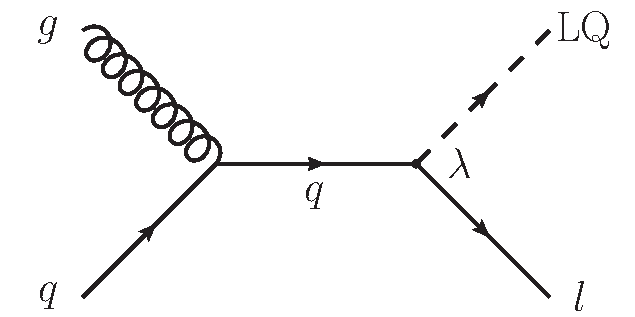
\includegraphics[width=\textwidth]{tex/theory/fig/LO_FD_single_LQ_a}
    \caption{}
    \label{fig:feynman_LO_single_a}
  \end{subfigure}
  \begin{subfigure}[b]{0.45\textwidth}
    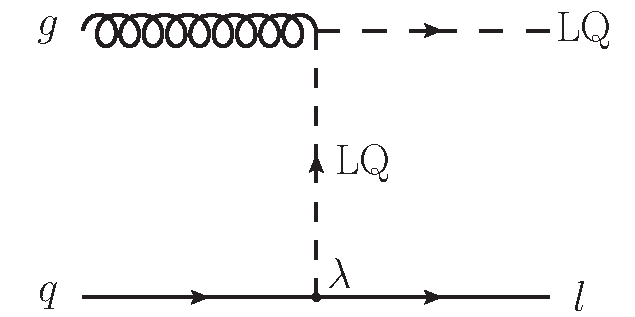
\includegraphics[width=\textwidth]{tex/theory/fig/LO_FD_single_LQ_b}
    \caption{}
    \label{fig:feynman_LO_single_b}
  \end{subfigure}
  \caption{Feynman diagrams for the single production of scalar leptoquarks.}
  \label{fig:feynman_LO_single}
\end{figure}

Because leptoquarks are $\text{SU}(3)_{C}$ color triplets, 
leptoquark pair production in $pp$ collisions occurs primarily
through quark-antiquark annihilation and gluon-gluon fusion
\cite{lq-vector-to-gluons,lq-scalar-hadron-colliders}, with gluon-gluon fusion dominating \cite{belyaev}.
These contributions from bosonic couplings ensure that low energy constraints
on the fermionic couplings do not constrain scattering cross sections.
As a result, searches for the pair production of scalar leptoquarks
are given as limits on leptoquark mass only, independent of any coupling
\cite{pair-lq-D0,pair-lq1-ATLAS,pair-lq2-ATLAS,pair-lq-CMS}.
In addition, leptoquark pair
production cross sections are predicted to be significantly larger
than those of leptoquark single production
for leptoquarks with mass less than 1.2 TeV \cite{belyaev}.
Figure \ref{fig:feynman_LO_LQ_pair} shows six examples of leading order leptoquark single production
Feynman diagrams.  It is notable that Figure \ref{fig:feynman_LO_LQ_pair_b} in particular
features a $t$-channel lepton exchange, which implies that its cross section will be proportional
to $\lambda^2$.

\begin{figure}
  \centering
  \begin{subfigure}[b]{0.45\textwidth}
    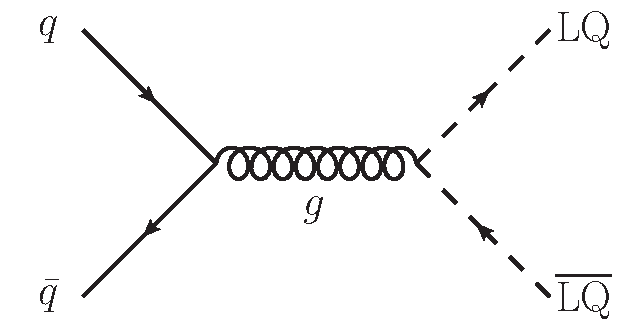
\includegraphics[width=\textwidth]{tex/theory/fig/LO_FD_LQ_pair_a}
    \caption{}
    \label{fig:feynman_LO_LQ_pair_a}
  \end{subfigure}
  \begin{subfigure}[b]{0.45\textwidth}
    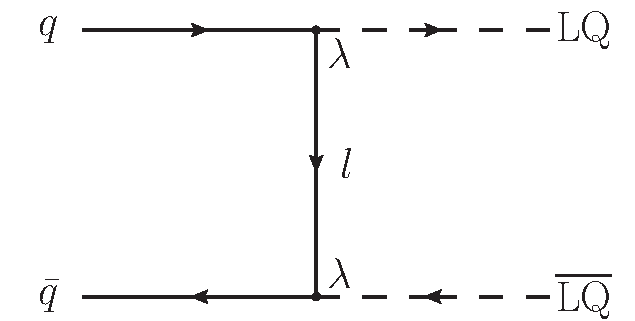
\includegraphics[width=\textwidth]{tex/theory/fig/LO_FD_LQ_pair_b}
    \caption{}
    \label{fig:feynman_LO_LQ_pair_b}
  \end{subfigure}

  \begin{subfigure}[b]{0.45\textwidth}
    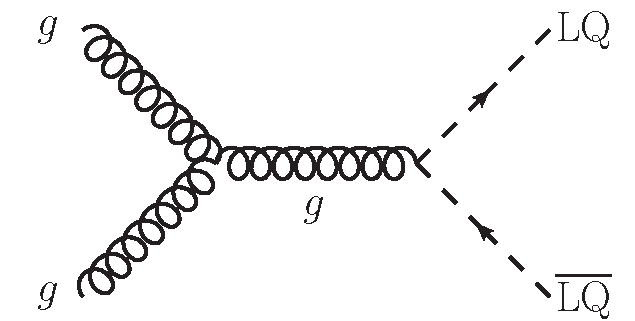
\includegraphics[width=\textwidth]{tex/theory/fig/LO_FD_LQ_pair_c}
    \caption{}
    \label{fig:feynman_LO_LQ_pair_c}
  \end{subfigure}
  \begin{subfigure}[b]{0.45\textwidth}
    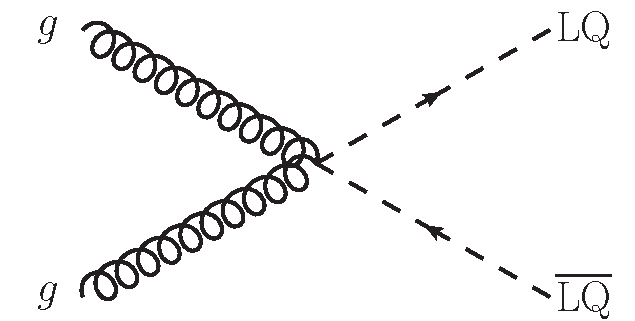
\includegraphics[width=\textwidth]{tex/theory/fig/LO_FD_LQ_pair_d}
    \caption{}
    \label{fig:feynman_LO_LQ_pair_d}
  \end{subfigure}

  \begin{subfigure}[b]{0.45\textwidth}
    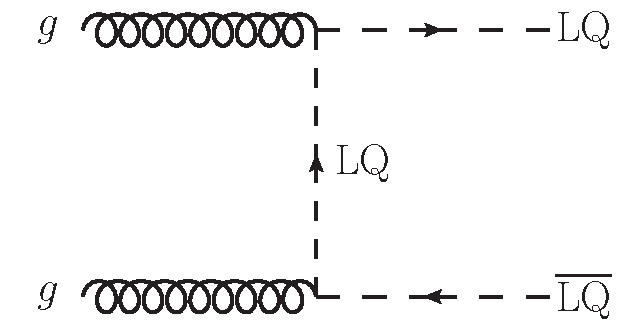
\includegraphics[width=\textwidth]{tex/theory/fig/LO_FD_LQ_pair_e}
    \caption{}
    \label{fig:feynman_LO_LQ_pair_e}
  \end{subfigure}
  \begin{subfigure}[b]{0.45\textwidth}
    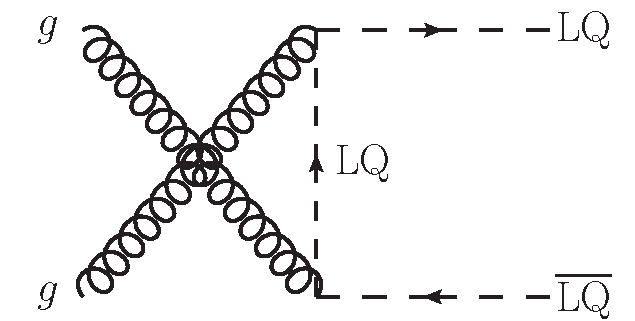
\includegraphics[width=\textwidth]{tex/theory/fig/LO_FD_LQ_pair_f}
    \caption{}
    \label{fig:feynman_LO_LQ_pair_f}
  \end{subfigure}
  \caption{Feynman diagrams for the pair production of scalar leptoquarks via
    quark-antiquark annihilation (a,b) and gluon-gluon fusion (c-e).
    The $t$-channel lepton exchange process shown in figure (b) has
    a cross section proportional to $\lambda^2$, which makes it
    model-dependent.  
  }
  \label{fig:feynman_LO_LQ_pair}
\end{figure}

Vector leptoquark pair production cross sections may be greater than those of their scalar
counterparts, but the values vary by as much as two orders of magnitude 
depending on the model and on the anomalous coupling parameters 
\cite{lq-vector-to-gauge-bosons-quartic-trilinear-2}. Scalar leptoquark pair 
production cross sections are generally model independent.
Michael Kr\u{a}mer et al. \cite{kramer} have written a tool 
to calculate the leading order and next to leading order 
(NLO)\nomenclature{NLO}{Next to leading order}
cross sections for scalar leptoquarks in 
$pp$ collisions for a given $\sqrt{s}$.  
The cross sections provided by this tool at 
at $\sqrt{s} = 7$~TeV and $\sqrt{s} = 8$~TeV 
are shown in Table \ref{tab:lq-xsection} as calculated using
the {\tt CTEQ6L1} parton density function 
(PDF)\nomenclature{PDF}{Parton density function}
\cite{cteq}.

\begin{table}
  \centering
  \begin{tabular}{c|cc|cc}
    & \multicolumn{2}{c|}{$\sqrt{s} = 7$~TeV} & \multicolumn{2}{c}{$\sqrt{s} = 8$~TeV} \\
    M(LQ) $[\text{GeV}]$ & $\sigma$(NLO) $[\text{pb}]$ & $\delta_{\text{PDF}}$ $[\text{pb}]$& $\sigma$(NLO) $[\text{pb}]$& $\delta_{\text{PDF}}$ $[\text{pb}]$ \\
    \hline\hline
    200  & $11.9$               & $0.986$               & $17.4$  & $1.24$  \\
    250  & $3.47$               & $0.372$               & $5.26$  & $0.487$  \\
    300  & $1.21$               & $0.158$               & $1.89$  & $0.214$  \\
    350  & $0.477$              & $0.728 \cdot 10^{-1}$ & $0.770$  & $0.102$ \\
    400  & $0.205$              & $0.357 \cdot 10^{-1}$ & $0.342$  & $0.520 \cdot 10^{-1}$ \\
    450  & $0.948 \cdot 10^{-1}$ & $0.185 \cdot 10^{-1}$ & $0.163$  & $0.278 \cdot 10^{-1}$ \\
    500  & $0.463 \cdot 10^{-1}$ & $0.996 \cdot 10^{-2}$ & $0.820 \cdot 10^{-1}$ & $0.115 \cdot 10^{-1}$ \\
    550  & $0.236 \cdot 10^{-1}$ & $0.558 \cdot 10^{-2}$ & $0.431 \cdot 10^{-1}$ & $0.893 \cdot 10^{-2}$ \\
    600  & $0.124 \cdot 10^{-1}$ & $0.321 \cdot 10^{-2}$ & $0.235 \cdot 10^{-1}$ & $0.530 \cdot 10^{-2}$ \\
    650  & $0.676 \cdot 10^{-2}$ & $0.190 \cdot 10^{-2}$ & $0.132 \cdot 10^{-1}$ & $0.322 \cdot 10^{-2}$ \\
    700  & $0.377 \cdot 10^{-2}$ & $0.114 \cdot 10^{-2}$ & $0.761 \cdot 10^{-2}$ & $0.200 \cdot 10^{-2}$ \\
    750  & $0.214 \cdot 10^{-2}$ & $0.700 \cdot 10^{-3}$ & $0.448 \cdot 10^{-2}$ & $0.126 \cdot 10^{-2}$ \\
    800  & $0.124 \cdot 10^{-2}$ & $0.437 \cdot 10^{-3}$ & $0.269 \cdot 10^{-2}$ & $0.810 \cdot 10^{-3}$ \\
    850  & $0.732 \cdot 10^{-3}$ & $0.276 \cdot 10^{-3}$ & $0.164 \cdot 10^{-2}$ & $0.527 \cdot 10^{-3}$ \\
    900  & $0.436 \cdot 10^{-3}$ & $0.176 \cdot 10^{-3}$ & $0.101 \cdot 10^{-2}$ & $0.347 \cdot 10^{-3}$ \\
    950  & $0.263 \cdot 10^{-3}$ & $0.113 \cdot 10^{-3}$ & $0.634 \cdot 10^{-3}$ & $0.231 \cdot 10^{-3}$ \\
    1000 & $0.160 \cdot 10^{-3}$ & $0.737 \cdot 10^{-4}$ & $0.401 \cdot 10^{-3}$ & $0.155 \cdot 10^{-3}$ \\
    1050 & $0.982 \cdot 10^{-4}$ & $0.483 \cdot 10^{-4}$ & $0.256 \cdot 10^{-3}$ & $0.105 \cdot 10^{-3}$ \\
    1100 & $0.606 \cdot 10^{-4}$ & $0.318 \cdot 10^{-4}$ & $0.165 \cdot 10^{-3}$ & $0.718 \cdot 10^{-4}$ \\
    1150 & $0.377 \cdot 10^{-4}$ & $0.210 \cdot 10^{-4}$ & $0.107 \cdot 10^{-3}$ & $0.492 \cdot 10^{-4}$ \\
    1200 & $0.235 \cdot 10^{-4}$ & $0.140 \cdot 10^{-4}$ & $0.696 \cdot 10^{-4}$ & $0.340 \cdot 10^{-4}$ \\
  \end{tabular}
  \caption{Next-to-leading order (NLO) pair production cross sections and PDF uncertainties 
    for scalar leptoquarks in $pp$ collisions at $\sqrt{s} = 7$~TeV (the LHC collision energy in 2010 and 2011) 
    and $\sqrt{s} = 8$~TeV (the LHC collision energy in 2012).
    Cross sections are given in units of pb ($1 \text{ b}= 10^{-28} \text{m}^2 = 10^{-24} \text{cm}^2$).
    In all cases, the renormalization and factorization scale is set to be equal to the 
    leptoquark mass. }
  \label{tab:lq-xsection}
\end{table}

\subsection{Leptoquark decays}
\label{sec:lq-decays}

Under the mBRW model, scalar and vector leptoquarks decay to a lepton-quark pair 
with total decay widths given by Equation \ref{eqn:lq-width} \cite{mBRW1,belyaev}.
\begin{equation}
  \begin{aligned}
    \Gamma_{\text{Scalar}} &= \sum_{i}\frac{\lambda_{i}^{2}}{16\pi}M_{\text{LQ}} \\
    \Gamma_{\text{Vector}} &= \sum_{i}\frac{\lambda_{i}^{2}}{24\pi}M_{\text{LQ}} 
  \end{aligned}
  \label{eqn:lq-width}
\end{equation}
In Equation \ref{eqn:lq-width}, $M_{\text{LQ}}$ corresponds to the mass of the
leptoquark, and $\lambda_i$ corresponds to the coupling between the leptoquark,
lepton, and quark for a given decay mode ($i$).  
The sum is taken over all leptoquark decay modes.
For a 1 TeV scalar leptoquark having a single decay mode with a coupling constant equal to that
of the electromagnetic interaction ($\lambda_{\text{em}} = 0.3$), the decay width is
approximately 1.8 GeV.  For a similar vector leptoquark, the width is approximately 1.2 GeV.
These widths are significantly less than experimental resolutions.

It should be noted that according to Equation \ref{eqn:lq-width}, 
leptoquark decay width is directly proportional to the coupling constant ($\lambda$),
and a small coupling constant corresponds to a long lived 
(narrow width) leptoquark.  While searches for the pair-production of 
scalar leptoquarks are generally treated independently of the coupling constant,
the coupling constant is generally assumed to be large enough so that the leptoquark
decays relatively promptly.  For example, a scalar leptoquark with $\lambda \sim 3 \cdot 10^{-8}$
has a decay length of approximately 1 meter.

Under the mBRW model, the branching fraction 
$\beta = \text{BR}(\text{LQ}\rightarrow\ell^{\pm} q)$
is required to have a value of either 0, 1/2, or 1.  This
can be seen in Table \ref{tab:lq-classification}.
$\beta$ may be treated with less rigidity if the 
assumption {\bf 3} of the BRW model is relaxed
(``leptoquarks couple {\it only} to Standard Model fermions and gauge bosons'').
For example, in the case of RPV SUSY, leptoquark-like squarks 
may decay to leptons, quarks, and other SUSY partners.
Many other examples exist for other models \cite{beta-1,beta-2,beta-3}.
In most experimental searches, $\beta$ is treated as a free parameter with the additional assumption that
$\text{BR}(\text{LQ}\rightarrow\ell^{\pm} q) + \text{BR}(\text{LQ}\rightarrow\nu q) = 1$.

This additional assumption leads to three separate final
states for leptoquark pair production:
two charged leptons and two quarks; one charged lepton, one neutrino, and two quarks;
and two neutrinos and two quarks.
For experimental searches, this corresponds to three different analysis final states:
two charged leptons and two jets;
one charged lepton, two jets, and missing transverse energy;
and two jets and missing transverse energy.
These final states and their branching ratios are listed
in Table \ref{tab:lq-decay}.  The leading order 
Feynman diagrams for the case when first generation leptoquarks decay to an electron or electron neutrino
are shown in Figure \ref{fig:feynman_LQ_decay}.

\begin{table}
  \renewcommand{\arraystretch}{1.5}
  \centering
  \begin{tabular}{l|l}
    Decay mode & Branching fraction \\
    \hline\hline
    $\text{LQ}\overline{\text{LQ}} \rightarrow \ell^{-}q\ell^{+}\overline{q}$ & $\beta^2$ \\ 
    $\text{LQ}\overline{\text{LQ}} \rightarrow \ell^{-}q\overline{\nu}_{\ell}\overline{q}', \nu_{\ell} q' \ell^{+}\overline{q}$ & $2\beta(1-\beta)$ \\ 
    $\text{LQ}\overline{\text{LQ}} \rightarrow \nu_{\ell}q \overline{\nu}_{\ell}\overline{q}$ & $(1-\beta)^2$ \\ 
  \end{tabular}
  \caption{List of the three distinct final states for pair produced leptoquarks
    and their associated branching fractions.  $\beta$ is defined such that 
    $\beta = \text{BR}(\text{LQ}\rightarrow\ell^{\pm} q)$.}
  \label{tab:lq-decay}
  \renewcommand{\arraystretch}{1.0}
\end{table}

\begin{figure}
  \centering
  \begin{subfigure}[b]{\textwidth}
    \begin{subfigure}[b]{0.45\textwidth}
      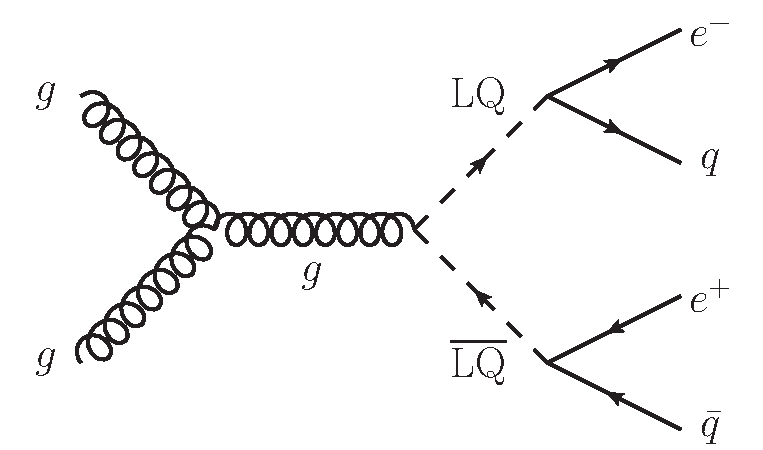
\includegraphics[width=\textwidth]{tex/theory/fig/LQ_pair_decay_eejj}
    \end{subfigure}
    \begin{subfigure}[b]{0.5\textwidth}
      $\text{BR}(\text{LQ}\overline{\text{LQ}} \rightarrow e^{-}qe^{+}\overline{q}) = \beta^2$
    \end{subfigure}
    \caption{\eejj~channel}
    \label{fig:feynman_LO_LQ_pair_eejj}
  \end{subfigure}
  
  \begin{subfigure}[b]{\textwidth}
    \begin{subfigure}[b]{0.45\textwidth}
      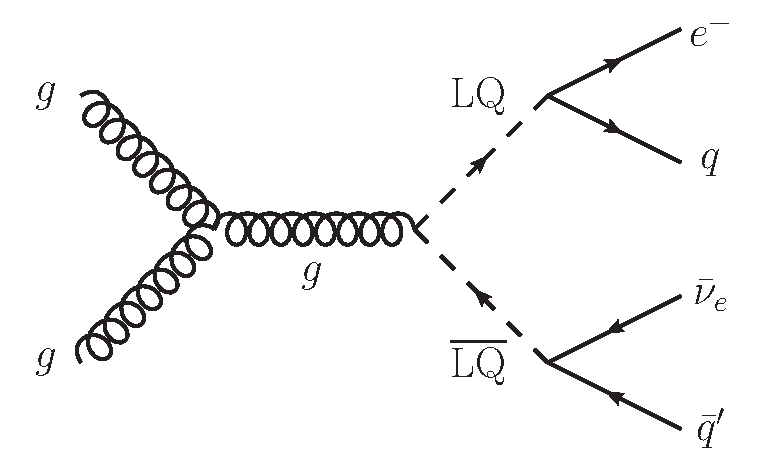
\includegraphics[width=\textwidth]{tex/theory/fig/LQ_pair_decay_enujj}
    \end{subfigure}
    \begin{subfigure}[b]{0.5\textwidth}
      $\text{BR}(\text{LQ}\overline{\text{LQ}} \rightarrow e^{-}q\overline{\nu}_{e}\overline{q}', \nu_{e} q' e^{+}\overline{q}  ) = 2\beta (1-\beta)$
    \end{subfigure}
    \caption{\enujj~channel}
    \label{fig:feynman_LO_LQ_pair_enujj}
  \end{subfigure}

  \begin{subfigure}[b]{\textwidth}
    \begin{subfigure}[b]{0.45\textwidth}
      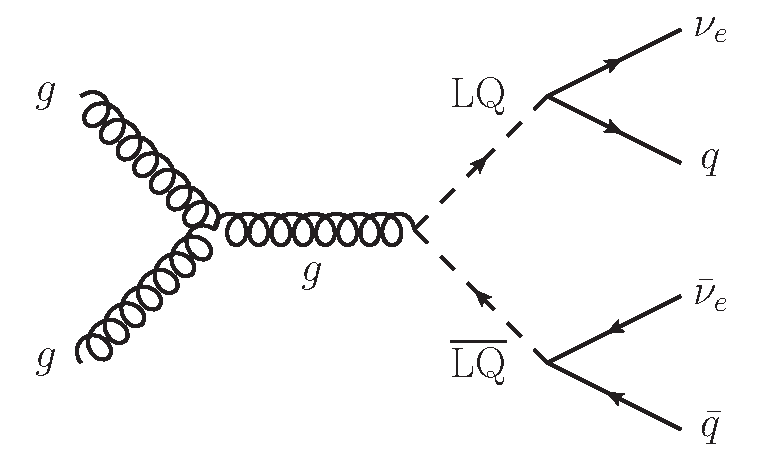
\includegraphics[width=\textwidth]{tex/theory/fig/LQ_pair_decay_nunujj}
    \end{subfigure}
    \begin{subfigure}[b]{0.5\textwidth}
      $\text{BR}(\text{LQ}\overline{\text{LQ}} \rightarrow \nu_{e}q \overline{\nu}_{e}\overline{q}) = (1-\beta)^2$
    \end{subfigure}
    \caption{\nunujj~channel}
    \label{fig:feynman_LO_LQ_pair_nunujj}
  \end{subfigure}
  \caption{Possible final states for a decay of a pair of first-generation scalar leptoquarks.
    $q$ denotes either an up or down quark.}
  \label{fig:feynman_LQ_decay}
\end{figure}

\subsection{Current limits}

Experimental limits on leptoquark states are obtained by
indirect searches and direct searches.  The indirect
limits are calculated from bounds on leptoquark-induced                                                     
four-fermion interactions, which come from low
energy experiments, or from collider experiments below threshold.
For a more detailed overview of indirect limits on leptoquarks,
the reader is referred to Reference \cite{pdg}.
The direct limits on leptoquarks are calculated from their production
cross section at colliders.  Direct limits on first generation
leptoquarks are discussed below.

The most stringest limits on the mass of first generation leptoquarks
from single production searches 
are produced by HERA experiments: ZEUS and H1.
The most recent limits for all 14 of the first generation
BRW leptoquarks are shown in Figure \ref{fig:hera-brw} \cite{zeus}.
These $\lambda$-dependent and model-dependent limits were obtained
using $ep$ collisions recorded with the ZEUS detector.
Comparable limits were obtained by H1 \cite{h1}.

\begin{figure}
  \centering
  \begin{subfigure}[b]{0.49\textwidth}
    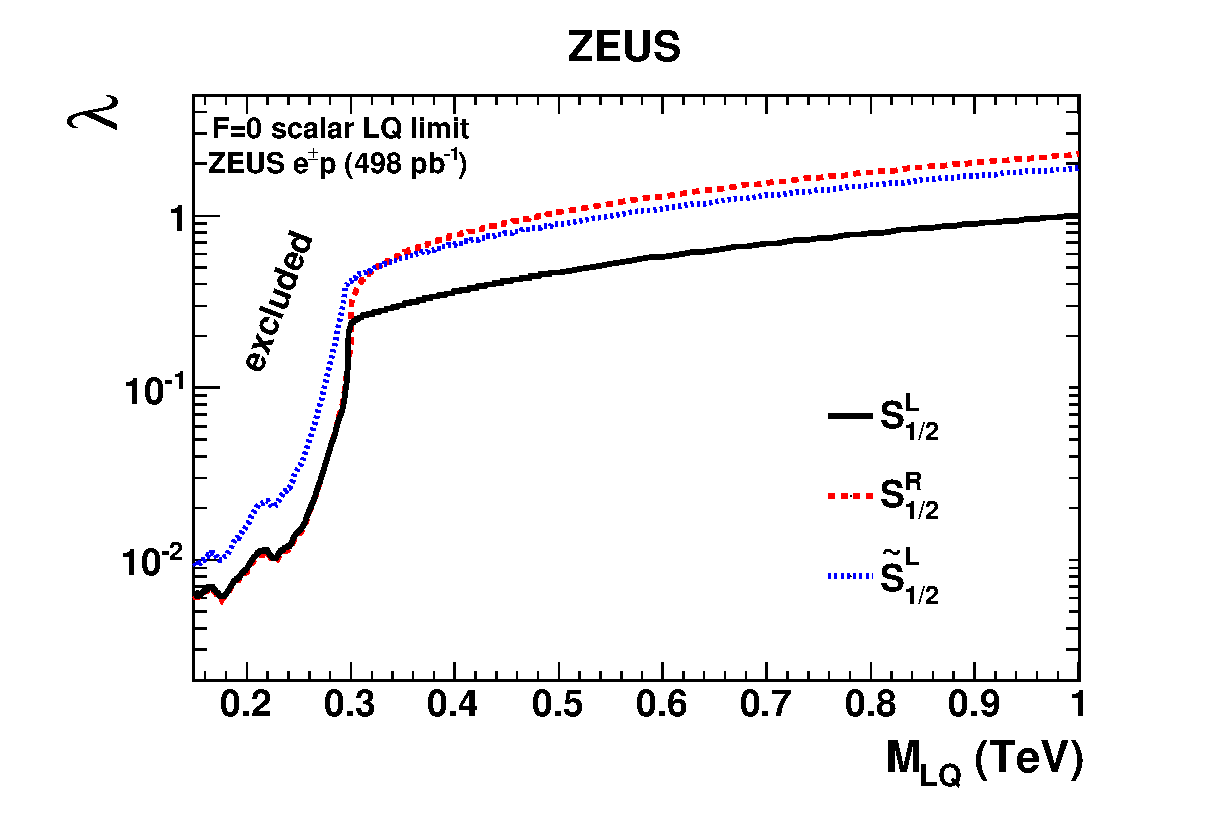
\includegraphics[width=\textwidth]{tex/theory/fig/limits/DESY-12-077_12.eps}
    \caption{}
    \label{fig:hera-F0S}
  \end{subfigure}
  \begin{subfigure}[b]{0.49\textwidth}
    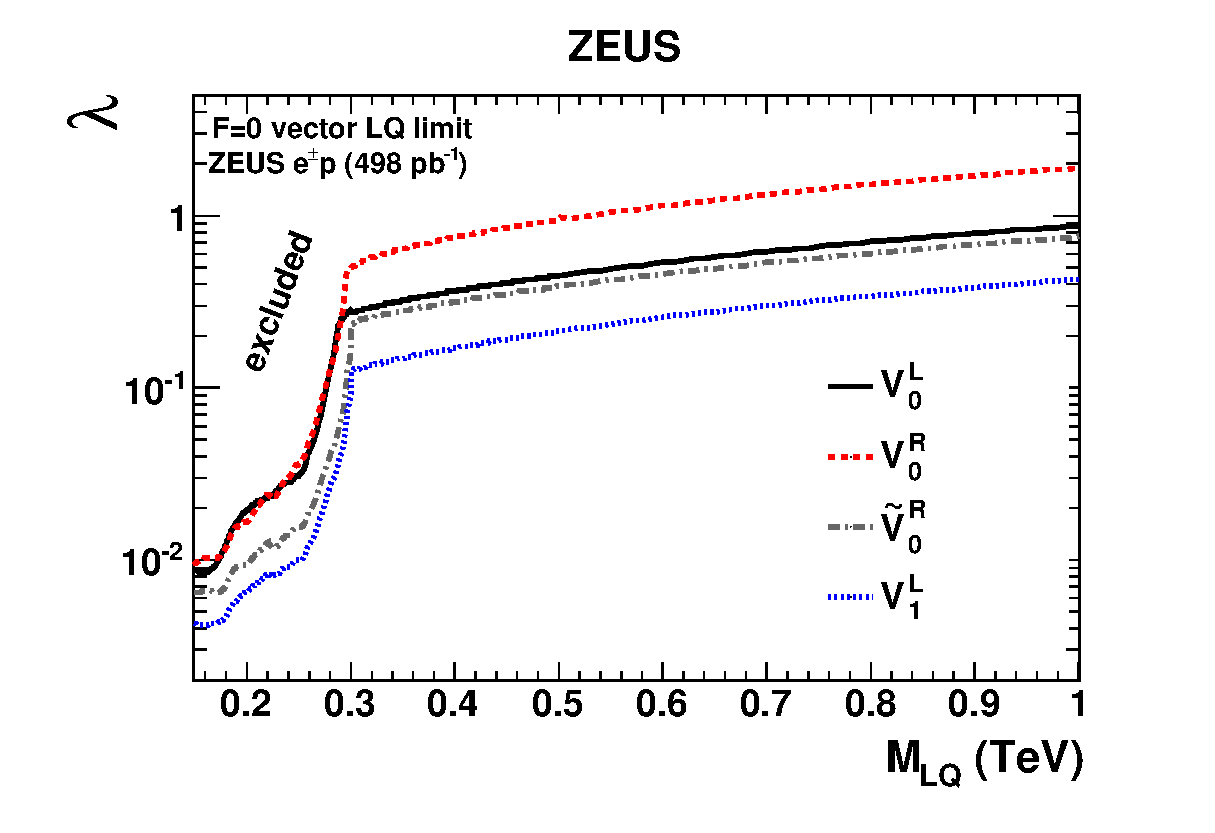
\includegraphics[width=\textwidth]{tex/theory/fig/limits/DESY-12-077_13.eps}
    \caption{}
    \label{fig:hera-F0V}
  \end{subfigure}
 \begin{subfigure}[b]{0.49\textwidth}
    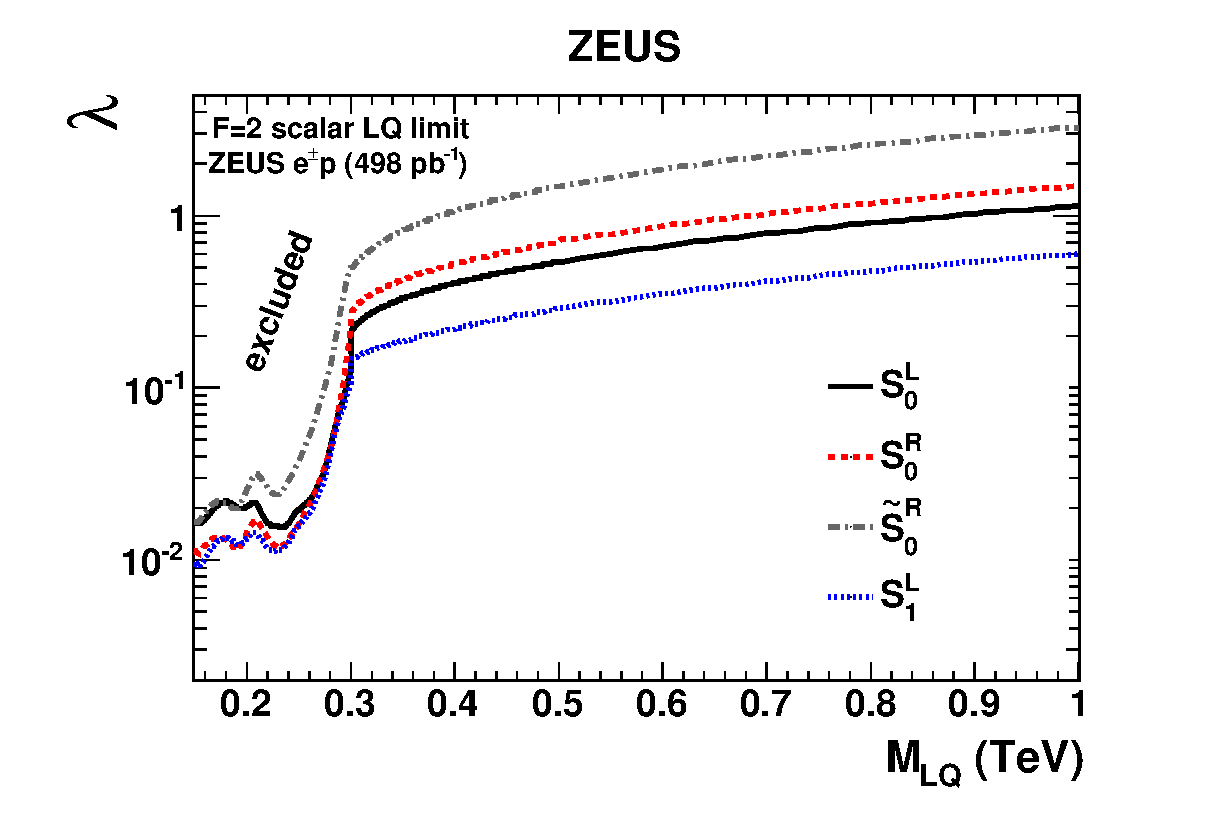
\includegraphics[width=\textwidth]{tex/theory/fig/limits/DESY-12-077_14.eps}
    \caption{}
    \label{fig:hera-F2S}
  \end{subfigure}
  \begin{subfigure}[b]{0.49\textwidth}
    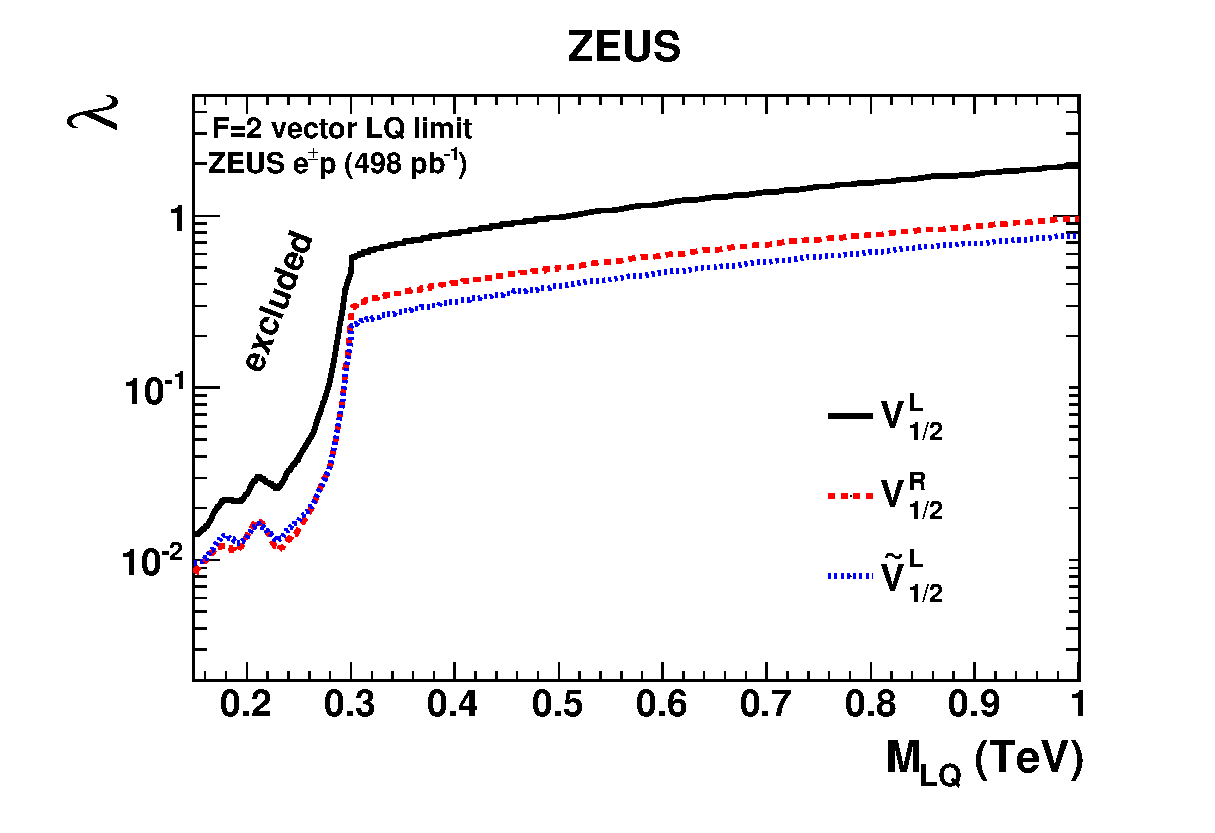
\includegraphics[width=\textwidth]{tex/theory/fig/limits/DESY-12-077_15.eps}
    \caption{}
    \label{fig:hera-F2V}
  \end{subfigure}
  \caption{95\% confidence level exclusion limits for all 14 of the 
    first generation leptoquarks described by the BRW model. 
    These limits were obtained using electron-proton and positron-proton
    collisions recorded with the ZEUS detector.
    In each plot, the $x-$axis corresponds to leptoquark mass, and the
    $y-$axis corresponds to the leptoquark coupling $\lambda$.  
    Plot (a) shows results for the $F=0$ scalar leptoquarks.
    Plot (b) shows results for the $F=0$ vector leptoquarks.
    Plot (c) shows results for the $F=2$ scalar leptoquarks.
    Plot (d) shows results for the $F=2$ vector leptoquarks \cite{zeus}.}
  \label{fig:hera-brw}
\end{figure}

Prior to the release of the results contained in this thesis, 
the most stringent limits on the mass of first generation leptoquarks from pair production searches
came from the ATLAS experiment at the CERN LHC \cite{pair-lq1-ATLAS}.
Using roughly the earliest 20\% of the full 2011 LHC dataset, 
ATLAS excluded the production of first generation scalar leptoquarks
with masses less than 660 (607) GeV, when assuming the branching fraction
of a leptoquark to an electron or positron ($\beta$) was equal to 1.0 (0.5).
The CMS experiment (also at the CERN LHC) also produced limits on first generation
leptoquarks in a prior version of the analysis described by this thesis \cite{lq1-paolo,lq1-dinko}.
Using the 2010 LHC dataset, CMS excluded the production of first generation scalar leptoquarks
with masses less than 384 (340) GeV, when assuming the branching fraction
of a leptoquark to an electron or positron ($\beta$) was equal to 1.0 (0.5).
The exclusion limits on first generation leptoquarks in the leptoquark mass vs. $\beta$ plane
from the ATLAS search are shown in Figure \ref{fig:atlas-limit}.
The same results from the CMS search are shown in Figure \ref{fig:cms-limit}.
The ATLAS limit is more stringent than the CMS limit in part because the 2011 dataset used by the ATLAS
search was roughly 25 times the size of the 2010 dataset used by the CMS search.

\begin{figure}
  \centering
  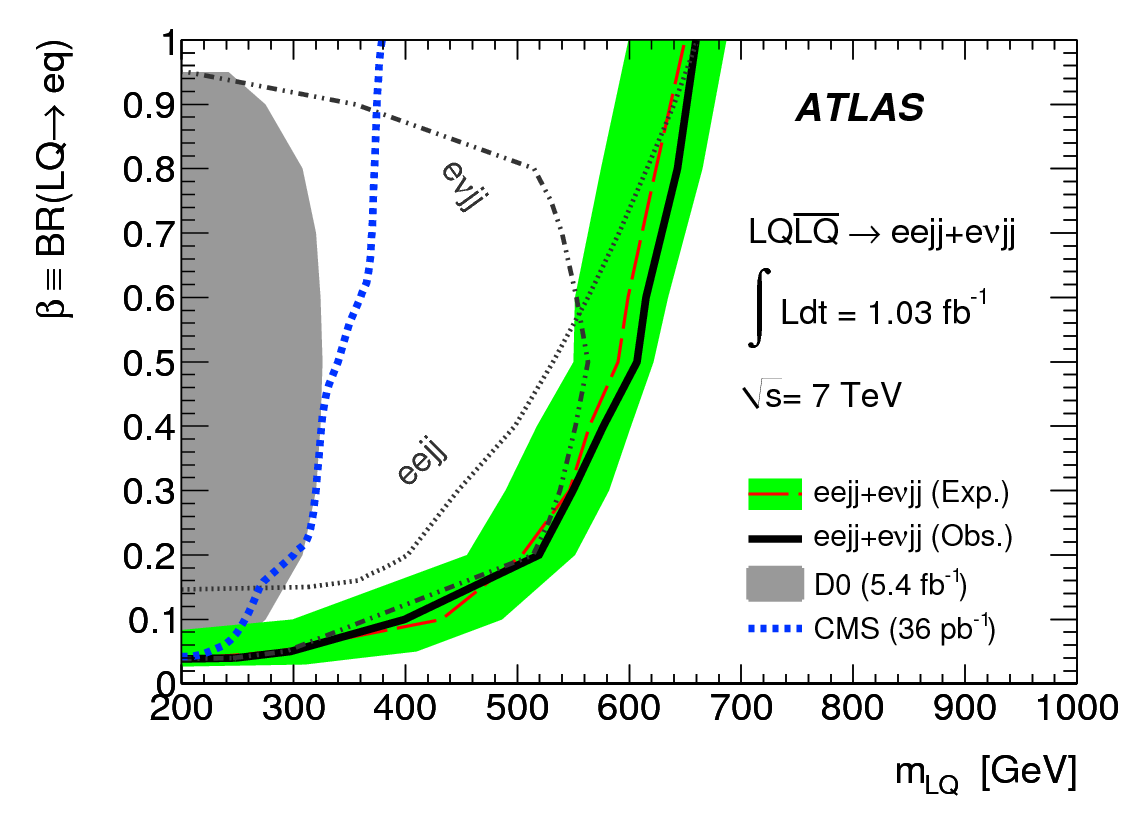
\includegraphics[width=0.80\textwidth]{tex/theory/fig/limits/ATLAS-2011.png}
  \caption{
    The expected and observed exclusion limits at 95\% CL on the first generation leptoquark
    hypothesis in the $\beta$ vs. mass plane using the central value of signal cross section for the
    individual \eejj~and \enujj~channels and their combination, from the ATLAS experiment in 2011.  The green expected
    limit uncertainty band represents the 95\% confidence interval.  The black solid line represents
    the observed combined exclusion limit.  
    The blue dashed line represents the observed exclusion limit from the CMS experiment in 2010 \cite{pair-lq1-ATLAS}.
  }
  \label{fig:atlas-limit}
\end{figure}

\begin{figure}
  \centering
  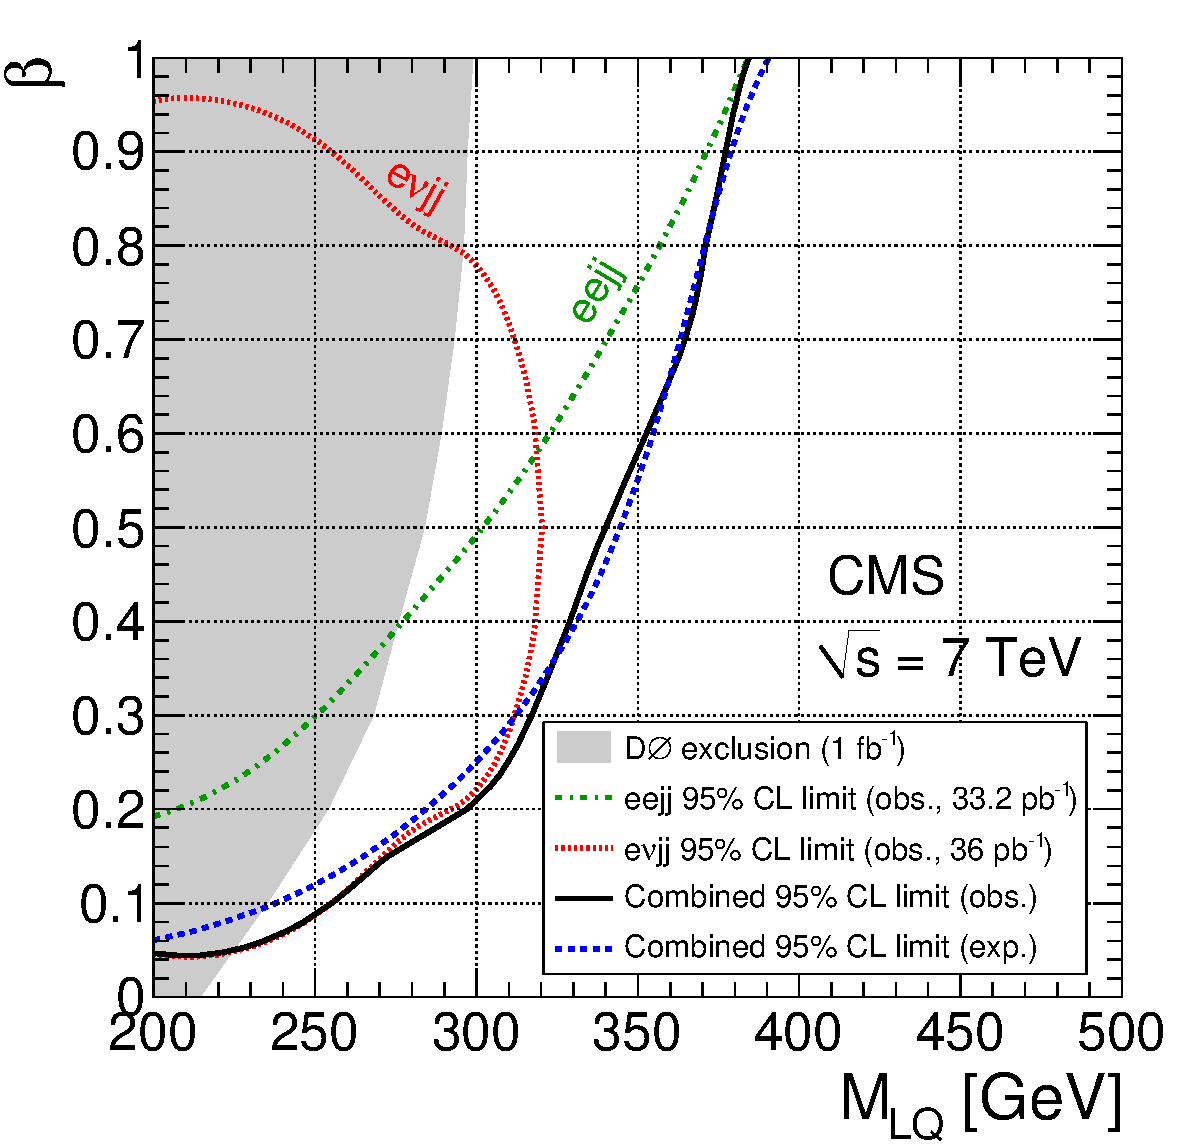
\includegraphics[width=0.80\textwidth]{tex/theory/fig/limits/CMS-2010.pdf}
  \caption{
    The expected and observed exclusion limits at 95\% CL on the first generation leptoquark
    hypothesis in the $\beta$ vs. mass plane using the central value of signal cross section for the
    individual \eejj~and \enujj~channels and their combination, from the CMS experiment in 2010.  
    The black solid line represents the observed combined exclusion limit, while the blue dashed line represents
    the expected exclusion limit.    
    The gray shaded area represents the observed exclusion limit from the D0 experiment at the Tevatron \cite{lq1-paolo,lq1-dinko}.
  }
  \label{fig:cms-limit}
\end{figure}
